\chapter{Groups}

\section{What is a Group?}

\begin{definition}[Groups]
  A set $G$ and an operation $\cdot$ form a \textbf{group} if and only if
  \begin{itemize}[noitemsep]
    \item \textbf{Closure} $\forall a,b \in G$, $a\cdot b \in G$
    \item \textbf{Associativity} $\forall a,b,c, \in G$, $(a \cdot b) \cdot c = a \cdot (b \cdot c)$
    \item \textbf{Existence of Indentity} $\exists a \in G$ such that $\forall b \in G$, $a \cdot b = b$.  Such $a$ is called the identity, denoted $\mathbb{I}$.
    \item \textbf{Existence of Inverse} $\forall a \in G$, $\exists a^{-1}$ such that $a^{-1} \cdot a = \mathbb{I}$.
  \end{itemize}
\end{definition}

Any types of objects can form the set.  Commonly we speak of these sets in terms of abstract numbers, for example addition on the set of real numbers, but this definition works on any collection of objects.


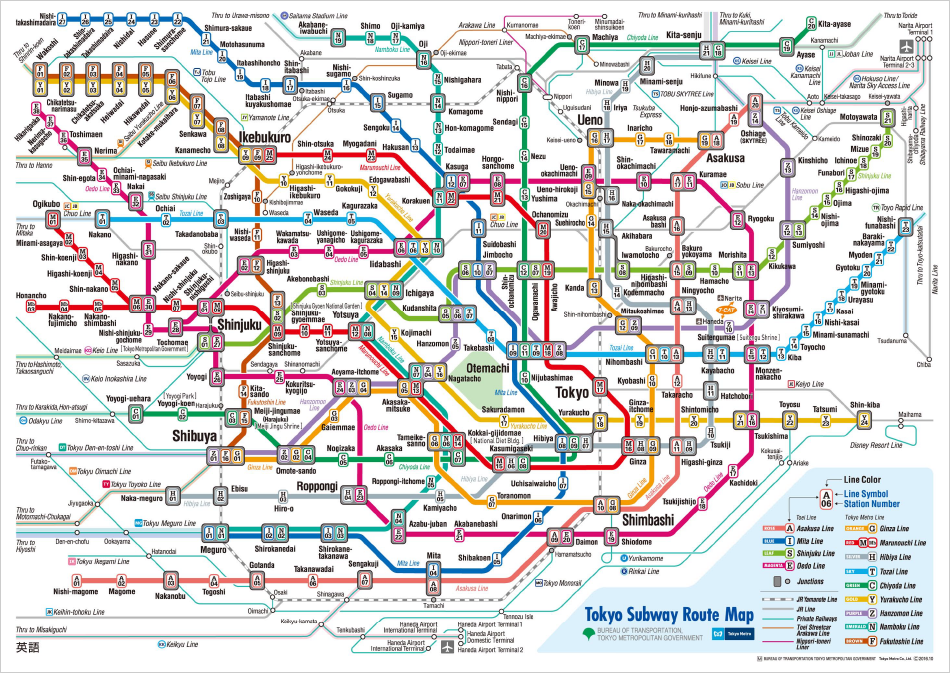
\includegraphics[width=\textwidth]{pics/tokyo_subway.png}
For example, take each path, even disjointed ones, you can take on the Tokyo subway as the element of a set. One element would be Shibuya $\rightarrow$ Shinjuku, another Shinjuku $\rightarrow$ Shibuya, yet another Asakusa $\rightarrow$ Akihabara.  Let's just assume specifying start and end points is enough to make the path deterministic, even though it totally isn't, especially for very confused tourists.  Once I have gone from one station to a new one, I can travel from the new station to a third.  Putting these two paths together is our composition operator $\cdot$.  For example, Ikebukuro$\rightarrow$ Shinjuku $\cdot$ Shinjuku $\rightarrow$ Shibuya .

If we only composed elements whose end points matched the start of the next, we would have a \textit{groupoid} rather than a group.   But we don't actually need the constraint that the end of one element has to match the start of the next.  For example, I could get into Tokyo at Shinjuku, then travel to Shibuya.  After wandering around and spending my year's worth of clothing budget, I might hop back on the subway at Harajuku to travel to Akihabara for some night life.  That element would be Shinjuku$\rightarrow$Shibuya$\cdot$ Harajuku$\rightarrow$Akihabara.  While Shibuya and Harajuku are fairly close together, what if I ran the Tokyo marathon? Or took an express bus to the airport, only to find out my plane was canceled and take the train back into the city?  I can compose paths arbitrarily far apart.

Let's work through requirements in the definition of a group.  Does this group obey \textbf{closure}?  Well, by combining any two routes in the metro, we still can't get anywhere the metro doesn't travel, so the composition will still be in the group.

How about \textbf{Associativity}?  The parentheses don't change how we will traverse the route, since we still tranverse the route left to right.  The parentheses only change how we \textit{plan} our route.  No matter how we plan, the start and end points will still end up being the same, and we will still have the same group object.

\textbf{Indentity}? One time in Akihabara, I couldn't figure out how to get to the locker where I stashed my luggage, so I had to pay to walk in one entrance and out a different exit.  In essence, I used the metro, but I didn't go anywhere.  I just applied the identity operation.  That exists for any station.

\textbf{Existance of Inverse}?  At least in this particular Metro, trains run both ways. This is a particularily nice feature for confused tourists who just jumped on a train before checking if it was the correct one. If I can travel A$\rightarrow$B, then I can travel B$\rightarrow$A.  If I combine those two paths, I get A$\rightarrow$B$\rightarrow$A = A$\rightarrow$A = I.

\section{Subgroups}

* Proper Subgroups

* Normal Subgroups

\section{Cosets of Subgroups}


\section{Quotient Groups}

* Conjugacy class
